\documentclass[12pt, a4paper, oneside]{article}
\usepackage{graphicx}
\usepackage{arial}
\renewcommand{\familydefault}{\sfdefault}
\usepackage[T1]{fontenc}
\usepackage[polish]{babel}
\usepackage[utf8]{inputenc}
\usepackage{lmodern}
\usepackage[left=2cm,right=2cm,top=2cm,bottom=2cm]{geometry}
\selectlanguage{polish}

\begin{document}
\section{Analiza budowy drzewa decyzyjnego}
\begin{figure}[h!]
\centering
\caption{Rozkład wektorów decyzyjnych dla r = 1}
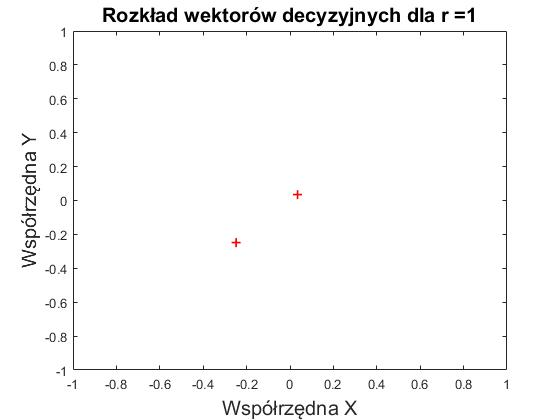
\includegraphics[scale=0.65]{pics/f1}
\end{figure}
\begin{center}
2 centroidy rozmieszczone symetrycznie względem punktu P = (0,0).
\end{center}
\begin{figure}[h!]
\centering
\caption{Rozkład wektorów decyzyjnych dla r = 2}
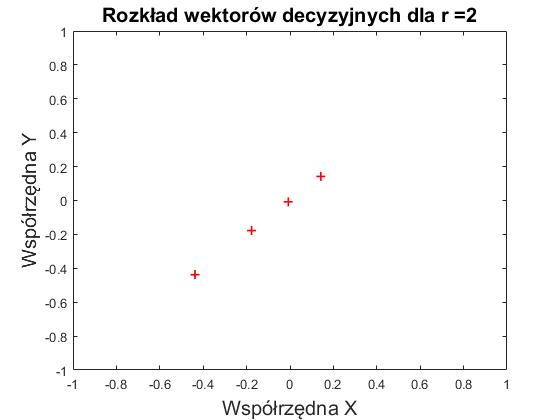
\includegraphics[scale=0.65]{pics/f2}
\end{figure}
\begin{center}
4 centroidy rozmieszczone współliniowo względem punktu P = (0,0).
\end{center}
\clearpage
\begin{figure}[h!]
\centering
\caption{Rozkład wektorów decyzyjnych dla r = 3}
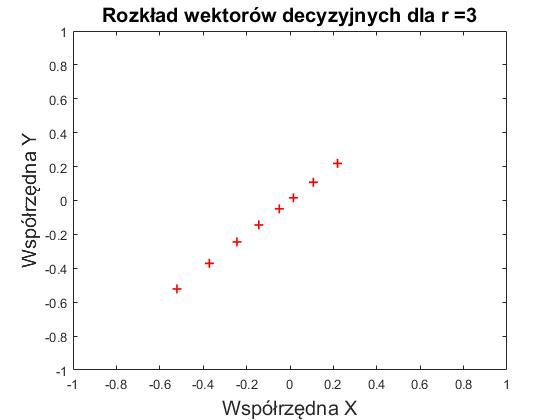
\includegraphics[scale=0.65]{pics/f3}
\end{figure}
\begin{center}
8 centroidów rozmieszczonych współliniowo względem punktu P = (0,0).
\end{center}
\begin{figure}[h!]
\centering
\caption{Rozkład wektorów decyzyjnych dla r = 4}
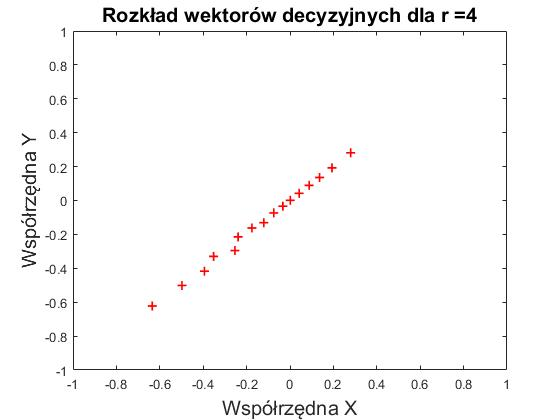
\includegraphics[scale=0.65]{pics/f4}
\end{figure}
\begin{center}
16 centroidy rozmieszczonych współliniowo względem punktu P = (0,0).
\end{center}
\clearpage
\begin{figure}[h!]
\centering
\caption{Rozkład wektorów decyzyjnych dla r = 5}
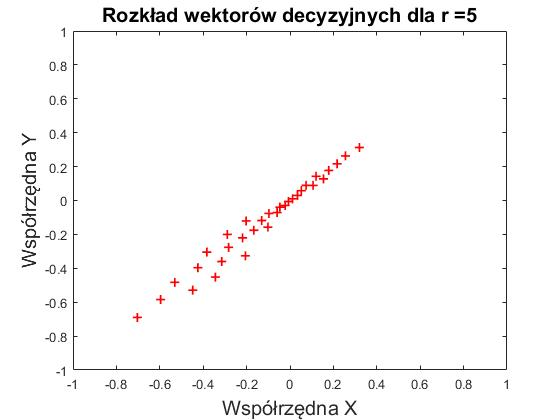
\includegraphics[scale=0.65]{pics/f5}
\end{figure}
\begin{center}
32 centroidy, utrata współliniowości, lekkie zagęszczenie wokół punktu P = (0,0).
\end{center}
\begin{figure}[h!]
\centering
\caption{Rozkład wektorów decyzyjnych dla r = 6}
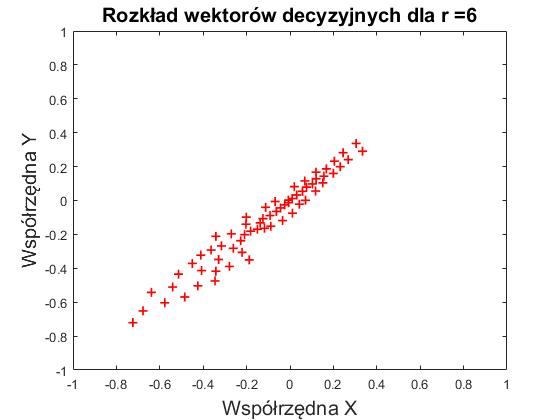
\includegraphics[scale=0.65]{pics/f6}
\end{figure}
\begin{center}
64 centroidy, dalsze zagęszczanie wokół punktu P = (0,0).
\end{center}
\clearpage
\begin{figure}[h!]
\centering
\caption{Rozkład wektorów decyzyjnych dla r = 7}
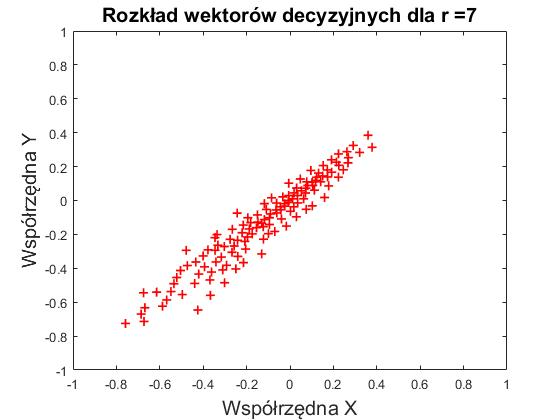
\includegraphics[scale=0.65]{pics/f7}
\end{figure}
\begin{center}
128 centroidów, duże zagęszczenie wokół punktu P = (0,0).\\W miarę oddalania się od punktu~P~zagęszczenie maleje.
\end{center}
\begin{figure}[h!]
\centering
\caption{Rozkład wektorów decyzyjnych dla r = 8}
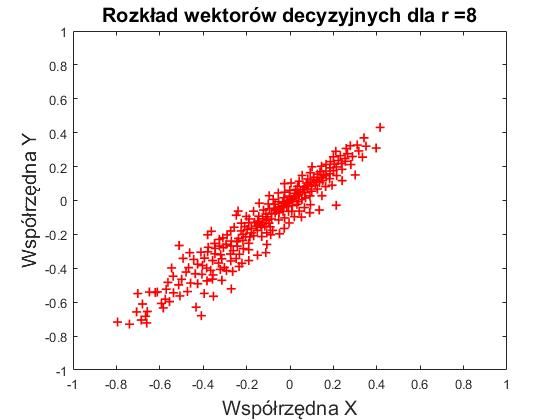
\includegraphics[scale=0.65]{pics/f8}
\end{figure}
\begin{center}
256 centroidów, bardzo duże zagęszczenie wokół punktu P = (0,0).\\W miarę oddalania się od punktu~P~zagęszczenie maleje.
\end{center}
\clearpage
\section{Badanie kodeka opartego o kwantyzację wektorową}
\begin{figure}[h!]
\centering
\caption{Wartość SNR w funkcji szybkości transmisji}
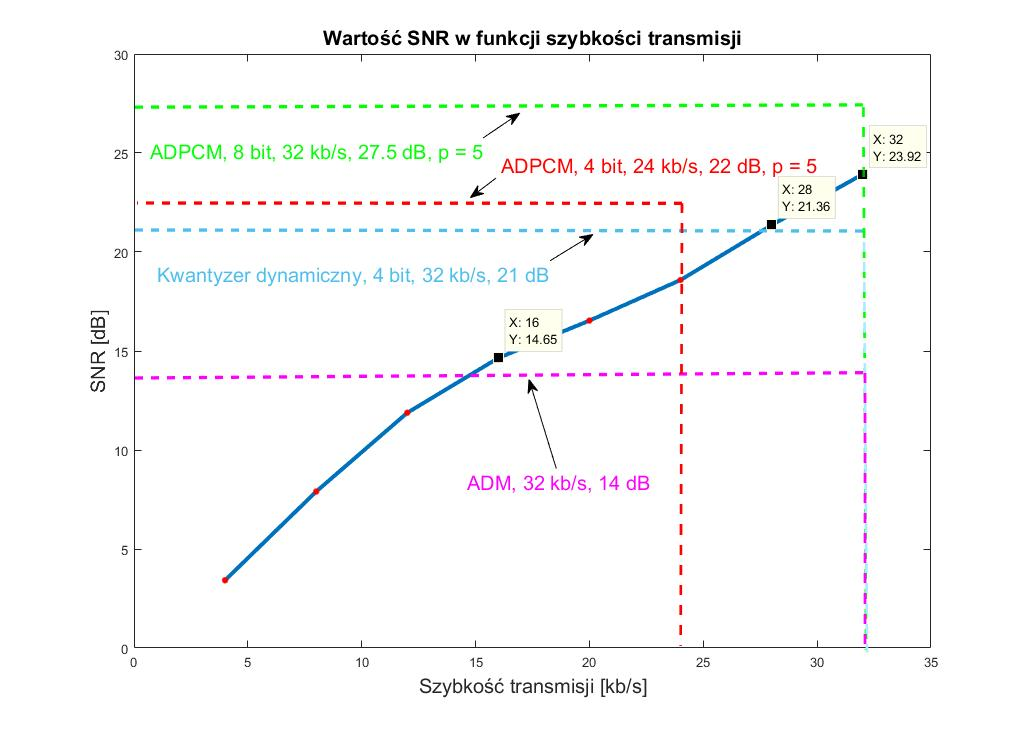
\includegraphics[scale=0.5]{pics/f9}
\end{figure}
\begin{table}[h!]
  \centering
  \caption{Porównanie kwantyzerów na podstawie rys. 9}
    \begin{tabular}{|c|c|c|c|c|c|}\hline
    Kwantyzer 1 & $v_t~[kb/s]$ & SNR [dB] & Kwantyzer 2 & $v_t~[kb/s]$ & SNR [dB] \\\hline
    Kwantyzer wekt. r = 4 & 16 & 14.6 & ADM & 32 & 14 \\\hline
    Kwantyzer wekt. r = 7 & 28 & 21.3 & Kwantyzer dyn. 4 bit & 32 & 21 \\\hline
    Kwantyzer wekt. r = 7 & 28 & 21.3 & ADPCM 4 bit & 24 & 22 \\\hline
    Kwantyzer wekt. r = 8 & 32 & 24 & ADPCM 8 bit & 32 & 27.5 \\\hline
    \end{tabular}%
  \label{tab:addlabel}%
\end{table}%
Kwantyzer wektorowy poddany został porównaniu z kwantyzerami ADM, dynamicznym 4 bitowym, ADPCM 4 bitowym oraz ADPCM 8 bitowym. Wszystkie badane kwantyzery zaznaczone zostały na rys. 9.\\
\indent W porównaniu z ADM lepszy okazał się kwantyzer wektorowy r = 4. Przy tym samym SNR na poziomie około 14 dB, oferuje zysk 16 kb/s na szybkości transmisji.\\
\indent Kwantyzer wektorowy r = 7 okazuje się także lepszy od kwantyzera dynamicznego 4 bitowego. Przy tym samym poziomie SNR = 21 dB, kwantyzer wektorowy wymaga szybkości niższej o 4 kb/s.\\
\indent ADPCM 4 bit jest korzystniejszy ze względu na wymaganą szybkość transmisji mniejszą o 4 kb/s niż w przypadku kwantyzera wektorowego r = 7. Różnica SNR wysosi 0.7 dB - również na korzyść ADPCM 4 bitowego.\\
\indent Porównując kwantyzer wektorowy r = 8 z ADPCM 8 bitowym wyższy SNR otrzymujemy dla ADPCM. Zysk wynosi 3.5 dB.
\clearpage
\section{Wnioski}
\begin{itemize}
\item Wraz ze wzrostem głębokości drzewa decyzyjnego obserwuje się zagęszczanie centroidów wokół punktu P = (0,0). Odsuwając się od niego, zauważyć można, że zagęszczenie maleje. Spełnia to oczekiwania dla sygnału mowy. Drzewo decyzyjne zostało zbudowane poprawnie.
\item W zestawieniu kwantyzera wektorowego okazał się on lepszy niż ADM oraz kwantyzer dynamiczny 4 bitowy. Przy podobnych poziomach SNR wymaga mniejszej szybkości transmisji.
\item ADPCM 4 bitowy jest lepszy niż kwantyzer wektorowy. Przy tym samym SQNR wymaga mniejszej szybkości transmisji.
\item W porównaniu ADPCM 8 bitowego wykorzystane zostało kryterium SNR przy tej samej szybkości transmisji. Kwantyzer wektorowy okazał się gorszy. Oferował SNR niższy o 3.5 dB.
\end{itemize}
\end{document}